\documentclass{exam}
\usepackage[exos]{main}

\title{Exercices}
\date{25 Avril 2024}
\author{Seconde 9}

\begin{document}
\maketitle
\thispagestyle{head}
\begin{questions}
\question $33$ est-il solution de l'inéquation $−x^2+2x−1 \leq 2x+3$ ?
\makeemptybox{1cm}
\question Résoudre l'inéquation $6x+6 \leq 7x - 13$. On donnera l'ensemble $\mathcal{S}$ des solutions sous la forme d'un intervalle.
\makeemptybox{5cm}
\question Soit la fonction $u$ dont la courbe représentative est donnée ci-après.

\begin{minipage}{0.45\textwidth}
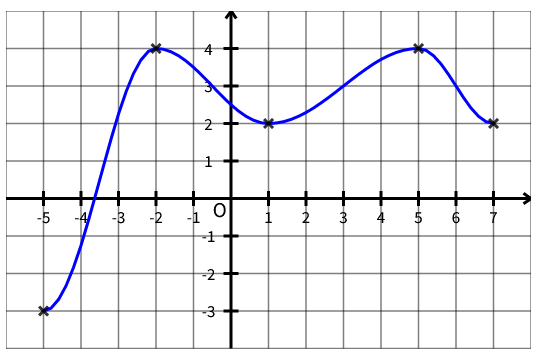
\includegraphics[width=\textwidth]{Revisions1.png}
\end{minipage}
\begin{minipage}{0.45\textwidth}
\begin{tikzpicture}
\tkzTabInit{$x$ /0.5, Variations de $u$ / 2}{,,};
\end{tikzpicture}
\end{minipage}
\begin{parts}
\part Compléter le tableau de variation.
\part Donner le minimum et le maximum de la fonction $u$.
\end{parts}
\makeemptybox{2cm}
\newpage
\question Soit $\function{f}{\left[-3;7\right]}{\R}{x}{4x^2-40x+112}$.
\begin{parts}
\part Montrer que pour tout $x \in \left[-3;7\right]$, nous avons
\begin{equation*}
f(x)=4(x-5)^2 + 12    
\end{equation*} 
\makeemptybox{3cm}
\part En déduire que pour tout $x \in \left[-3;7\right]$, $f(x) \geq 12$.
\makeemptybox{2cm}
\part Conclure que $12$ est le minimum de $f$ sur $\left[-3;7\right]$.
\makeemptybox{2cm}
\end{parts}
\question Soit $A(-2;-6)$; $B(7;x)$ avec $x$ un nombre réel quelconque.
\begin{parts}
\part Calculer la distance $AB$ quand $x = 0$.
\makeemptybox{2cm}
\part La distance $AB$ en fonction de $x$ est donnée par la fonction $g$. Donner l'expression de $g(x)$.
\makeemptybox{1cm} 
\end{parts}
\end{questions}
\end{document}